\documentclass[11pt, a4paper]{article}

%%% SST LAB PROTOCOLL PREAMBLE
%%% 2019
%%%%%%%%%%%%%%%%%%%%%%%%%%%%%%%


%%% PACKAGES
%%%%%%%%%%%%%%%%%%%%%%%%%%%

\usepackage[ngerman]{babel}

\usepackage[utf8]{inputenc}
\usepackage{amsmath}
\usepackage{pgfplots}
\usepackage{tikz}
\usepackage[many]{tcolorbox}
\usepackage{graphicx}
\graphicspath{ {./graphics/} }
\usepackage{pdfpages}
\usepackage{dashrule}
\usepackage{float}
\usepackage{siunitx}
\usepackage{trfsigns}
\usepackage{booktabs}
\usepackage[european]{circuitikz}
\usepackage{tcolorbox}

%%% DOCUMENT GEOMETRY
%%%%%%%%%%%%%%%%%%%%%%%%%%%

\usepackage{geometry}
\geometry{
 a4paper,
 total={0.6180339887498948\paperwidth,0.6180339887498948\paperheight},
 top = 0.1458980337503154\paperheight,
 bottom = 0.1458980337503154\paperheight
 }
\setlength{\jot}{0.013155617496424828\paperheight}
\linespread{1.1458980337503154}

\setlength{\parskip}{0.013155617496424828\paperheight} % paragraph spacing


%%% COLORS
%%%%%%%%%%%%%%%%%%%%%%%%%%%

\definecolor{red1}{HTML}{f38181}
\definecolor{yellow1}{HTML}{fce38a}
\definecolor{green1}{HTML}{95e1d3}
\definecolor{blue1}{HTML}{66bfbf}
\definecolor{hsblue}{HTML}{00b1db}
\definecolor{hsgrey}{HTML}{afafaf}

%%% CONSTANTS
%%%%%%%%%%%%%%%%%%%%%%%%%%%
\newlength{\smallvert}
\setlength{\smallvert}{0.0131556\paperheight}


%%% COMMANDS
%%%%%%%%%%%%%%%%%%%%%%%%%%%

% differential d
\newcommand*\dif{\mathop{}\!\mathrm{d}}

% horizontal line
\newcommand{\holine}[1]{
  	\begin{center}
	  	\noindent{\color{hsgrey}\hdashrule[0ex]{#1}{1pt}{3mm}}\\%[0.0131556\paperheight]
  	\end{center}
}

% mini section
\newcommand{\minisec}[1]{ \noindent\underline{\textit {#1} } \\}

% quick function plot
\newcommand{\plotfun}[3]{
  \vspace{0.021286\paperheight}
  \begin{center}
    \begin{tikzpicture}
      \begin{axis}[
        axis x line=center,
        axis y line=center,
        ]
        \addplot[draw=red1][domain=#2:#3]{#1};
      \end{axis}
    \end{tikzpicture}
  \end{center}
}

% box for notes
\newcommand{\notebox}[1]{

\tcbset{colback=white,colframe=green1!100!black,title=Note!,width=0.618\paperwidth,arc=0pt}

 \begin{center}
  \begin{tcolorbox}[]
   #1 
  \end{tcolorbox}
 
 \end{center} 
 
}

% box for equation
\newcommand{\eqbox}[2]{
	
	\tcbset{colback=white,colframe=green1!100!black,title=,width=#2,arc=0pt}
	
	\begin{center}
		\begin{tcolorbox}[ams align*]
				#1
		\end{tcolorbox}
		
	\end{center} 
	
}
% END OF PREAMBLE

\begin{document}

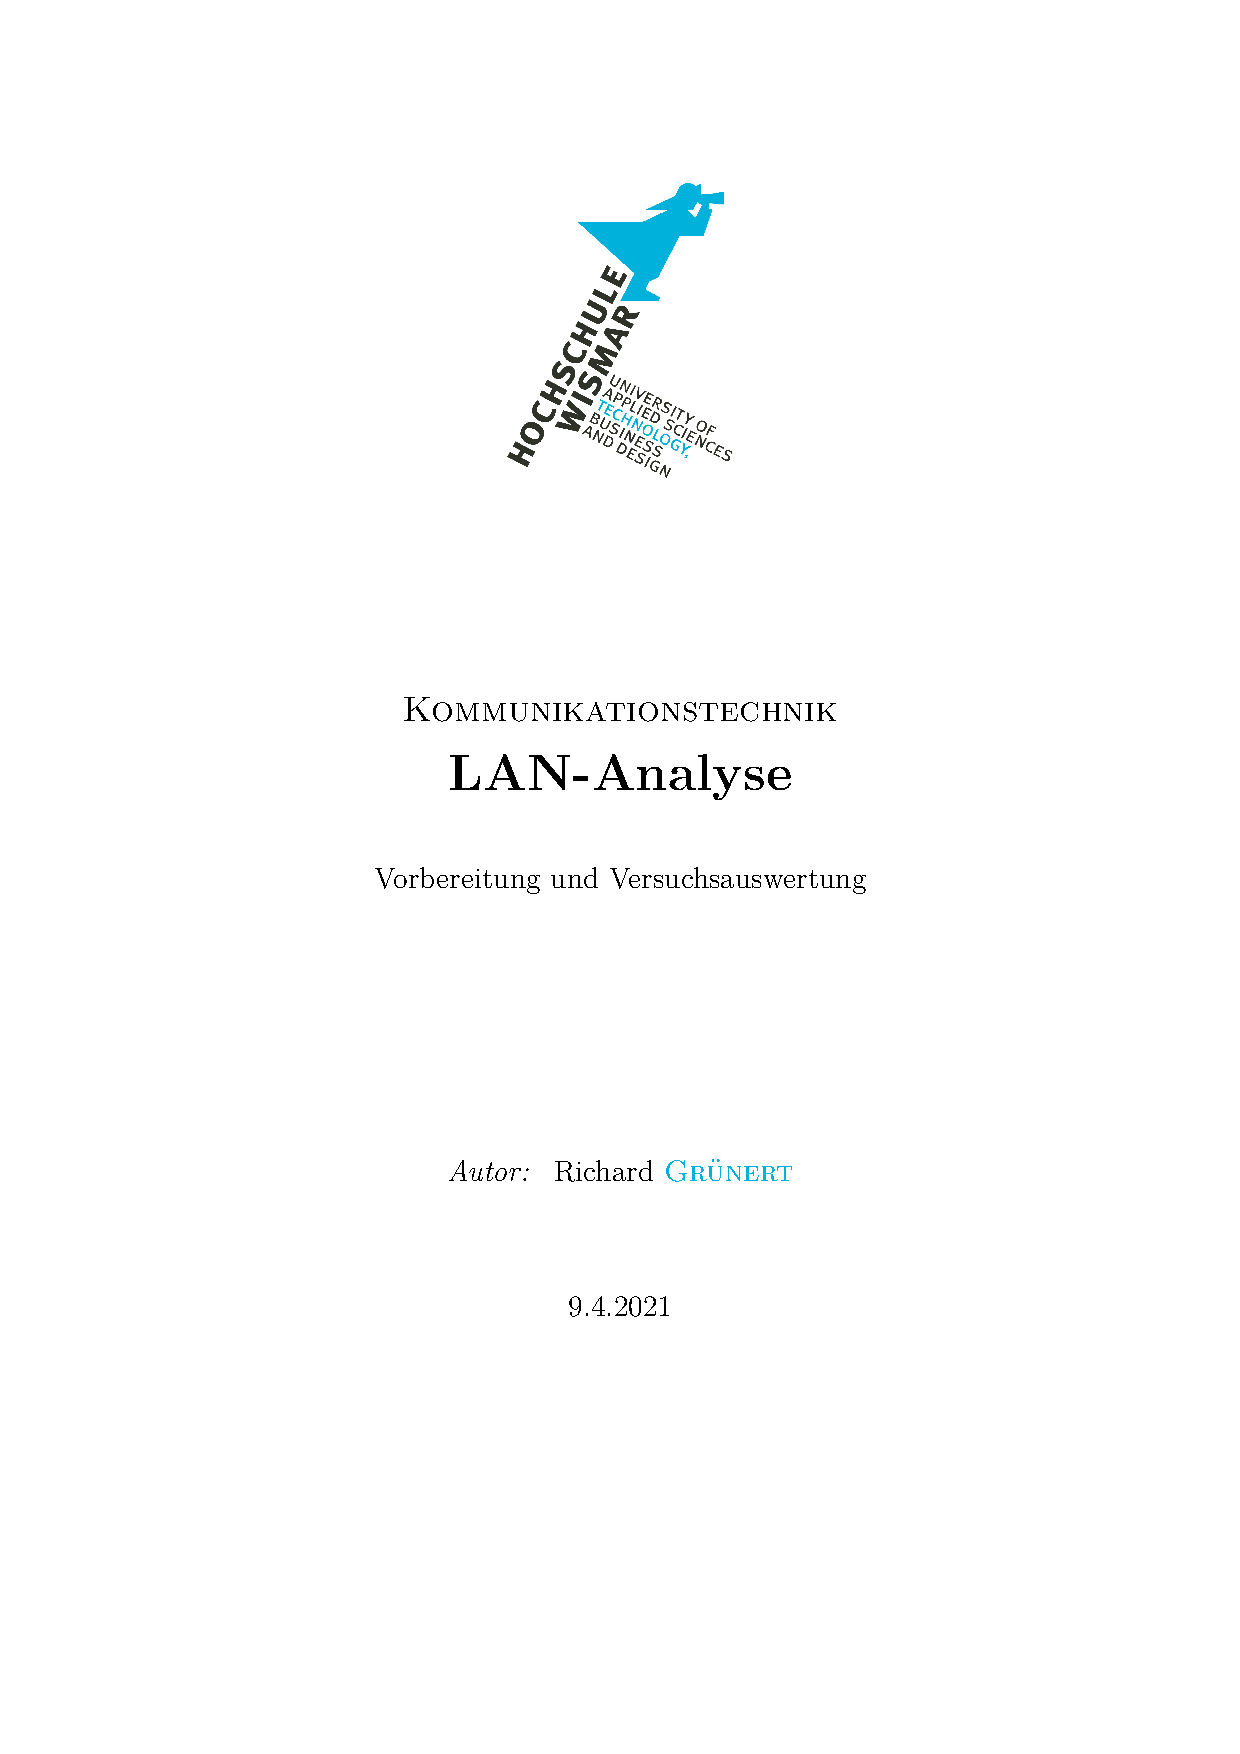
\includepdf{./titlepage/titlepage.pdf}

\section{Vorbereitungsaufgaben}

\subsection{OSI-Referenzmodell}
Das Ziel bei der Kommunikation zwischen zwei oder mehreren Geräten ist es, dass diese trotz Unterschiedlicher Hersteller und verschiedenen Technologien problemlos miteinander kommunizieren können. Um das zu erreichen, wurde das OSI-Referenzmodell (Open System Interconnection) entwickelt, welches die Kommunikation in 7 Teilaufgaben zerlegt, die als hierarchische Schichten (\emph{layers}) dargestellt werden können.
\begin{figure}[H]
\centering
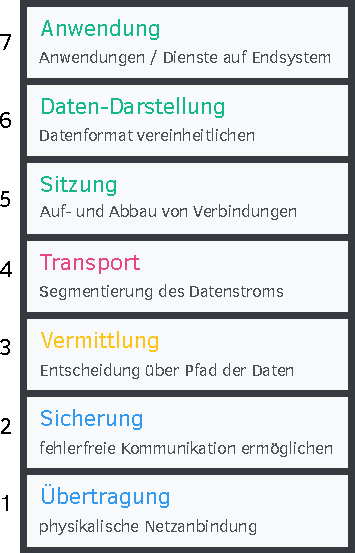
\includegraphics[width=0.382\textwidth]{graphics/a2.pdf}
\caption{Aufbau des OSI-Schichtenmodells mit (stark) vereinfachten Beschreibungen}
\end{figure}

\subsubsection{Schicht 1: Übertragung}
Die Übertragungsschicht (engl. \emph{physical layer}) beschreibt als unterste Ebene im OSI-Modell die physikalische Netzanbindung, d.h. die Umsetzung der Daten (Bits) in die messbare/empfangbare physikalische Größe und deren Form, also leitungsgebunden, Funkübertragung oder Lichtwellenübertragung, sowie Modulationsart und auch Kabel, Verbinder etc.

\subsubsection{Schicht 2: Sicherungsschicht}
Aufgabe der Sicherrungsschicht (engl. \emph{data-link layer}) ist die gewährleistung einer zuverlässigen, möglichst fehlerfreien Kommunikation. Sie regelt den Zugriff auf das Übertragungsmedium (Schicht 1) und führt Maßnahmen zu Flusskontrolle sowie Fehlerkontrolle durch Prüfsummen/Kanalkodierung durch. In dieser Schicht werden die Daten in \emph{Frames} eingeteilt (z.B. Ethernet-Frames (siehe \ref{A4.6}).
Schicht 2 wird unterteilt in \emph{LLC} und \emph{MAC}:
\begin{enumerate}
        \item[2b)] LLC, Logical Link Control\\
        \small Schnittstelle zwischen Layer 3 und MAC
        \item[2a)] MAC, Media Access Control\\
        \small regelt zugriff auf gemeinsames Medium
\end{enumerate}

\subsubsection{Schicht 3: Vermittlungs- / Netzwerkschicht}
Die Vermittlungsschicht (engl. \emph{network layer}) ist dafür zuständig, die Daten \emph{blockweise}, d.h. als sog. \emph{Pakete} zwischen den Endsystemen weiterzuvermitteln. Außerdem ist sie für die Stauvermeidung (Congestion Control), sowie die Wegsuche zwischen den Zwischensystemen / Netzwerkknoten (Routing) zuständig. Schicht 3 stellt weiterhin Netzwerkadressen bereit (z.B. IP), aktualisiert Routing-Tabellen und fragmentiert die Datenpakete.

\subsubsection{Schicht 4: Transportschicht}
In der Transportschicht (engl. \emph{transport layer}) wird der Datenstrom segmentiert, d.h. aufgeteilt auf mehrere Pakete (je nach Maximum Segment Size (MSS)), wobei jedem ein Header angefügt wird, welcher u.a. die Segmente nummeriert und das zugrundeliegende Protokoll (z.B. TCP oder UDP) sowie Ziel- und Quellport kennzeichnet. Mit Ziel und Quellport werden hier den segmentierten Datenpaketen Anwendungen auf den Endsystemen zugewiesen.

\subsubsection{Schicht 5: Sitzungsschicht}
Die Sitzungsschicht (engl. \emph{session layer}), auch Kommunikationsschicht, regelt den Auf- u. Abbau von Kommunikationssitzungen und ermöglicht die Wiederherstellung dieser nach Abbrüchen (Synchronisation).

\subsubsection{Schicht 6: Präsentationsschicht}
Die Präsentationsschicht (engl. \emph{presentation layer}) setzt die systemabhängige Darstellung der Daten (z.B. \textsc{ASCII}, \textsc{EBCDIC}) in eine unabhängige Form um, um den Datenaustausch zwischen unterschiedlichen Systemen zu ermöglichen. Außerdem fallen Aufgaben wie Datenkompression und -verschlüsselung in diese Ebene.

\subsubsection{Schicht 7: Applikationsschicht}
In der Anwendungsschicht befinden sich die Dienste der Anwendungsprogramme auf den jeweiligen Endsystemen. Hier findet man Protokolle wie HTTP, DNS, SMTP, FTP etc. Die Anwendungsprogramme selbst gehören nicht dazu.



\subsection{Netztopologien}
Unterschieden wird in \emph{physikalische} Topologien (realer Aufbau des Netzwerkes, physische Verbindungen, etc.) und \emph{logische} Topologien (prinzipielle Verbindungen der Teilnehmer ohne Details über physische Lage etc.). Je nach Topologie gibt es unterschiedliche Ausfallsicherheiten.

\subsubsection{Linie}

\begin{figure}[H]
\centering
\resizebox{0.618\textwidth}{!}{\import{graphics/}{top_linie.pdf_tex}}
\end{figure}

\subsubsection{Bus}

\begin{figure}[H]
\centering
\resizebox{0.618\textwidth}{!}{\import{graphics/}{top_bus.pdf_tex}}
\end{figure}

\subsubsection{Ring}

\begin{figure}[H]
\centering
\resizebox{0.618\textwidth}{!}{\import{graphics/}{top_ring.pdf_tex}}
\end{figure}

\subsubsection{Stern}

\begin{figure}[H]
\centering
\resizebox{0.618\textwidth}{!}{\import{graphics/}{top_stern.pdf_tex}}
\end{figure}

\subsubsection{Vollvermaschung}

\begin{figure}[H]
\centering
\resizebox{0.618\textwidth}{!}{\import{graphics/}{top_vollvermaschung.pdf_tex}}
\end{figure}


\pagebreak
\subsection{Unterschiede zwischen Ethernet und Token Ring}

\begin{multicols}{2}
\textbf{Ethernet}
\begin{itemize}
\item Bus-Topologie
\item Schreibt, wenn Bus frei
\item Bei Kollisionen $\rightarrow$ CSMA/Cx (Aufg. \ref{A4.4})
\end{itemize}

\columnbreak

\textbf{Token Ring}
\begin{itemize}
\item Stern-Topologie (log. Ring-Topologie)
\item Verwendet \emph{Token} als Signal für Schreibrechte
\item keine Kollisionen möglich
\end{itemize}
\end{multicols}


\subsection{Ethernetzugriffsverfahren}\label{A4.4}
Beim Ethernetzugriffsverfahren Carrier Sense Multiple Access \emph{CSMA} (Mehrfachzugriff mit Trägerprüfung) prüfen alle Teilnehmer das Übertragungsmedium auf dessen Zustand. Ist das Medium frei, kann gesendet werden, ist es belegt, wird gewartet bis es frei ist. Das Medium gilt als frei, wenn es für 96 Bitzeiten nicht belegt ist (z.B. $960 \, \si{\nano\second}$ bei $100 \, \si{\mega\bit\per\second}$).\\

Da nur lokal geprüft wird, kann bei der Ethernet- (Bus-) Übertragung eine Leitung durch Laufzeitunterschiede verschiedener Signale als frei erscheinen, obwohl auf der Leitung noch ein Signal \glqq wandert\grqq, wodruch fälschlicherweise gesendet wird und es es zu einer \emph{Kollision} kommt. Das CSMA-Verfahren wird demnach weiterhin unterschieden nach der Art der Kollisionsbehandlung.

\begin{description}
\item[Collision Avoidance (CA):] Ready to Send (RTS) Pakete gesendet bei Sendewunsch, Clear to Send (CTS) erhalten, falls frei. Genutzt in WLANs/Funk, da aufgrund der Reichweite keine komplette Überwachung des Mediums möglich.
\item[Collision Detection (CD):] Bei Kollision wird eine zufällige Zeit gewartet und dann erneut geprüft. Bei Überschreiten einer maximalen Anzahl von Versuchen tritt ein Fehler auf. Genutzt in LANs.
\item[Collision Resolution (CR):] Bei Kollision wird eine Prioritätsanalyse durchgeführt, wer zuerst angefangen hat, erhält das folgende Senderecht.
\end{description}


\subsection{Ablauf einer HTTP-Verbindung}
\subsubsection{Allgemein}\label{three_way}
Am Beginn einer HTTP-Verbinung steht der Verbindungsaufbau über das TCP-Protokoll und den sogenannten \emph{three-way-handshake}.
\begin{description}
\item[Schritt 1: SYN] Der Client schickt ein TCP-Paket mit gesetztem SYN-Flag, um eine Verbindung mit dem Empfänger zu initialisieren und seine Sequenznummer für die Nummerierung der Pakete anzugeben.
\item[Schritt 2: SYN-ACK] Der Server antwortet auf Schritt 1 zum einen mit einem ACK, um das Paket (SYN) zu bestätigen und zum anderen mit einem SYN, um seine eigene Sequenznummer anzugeben.
\item[Schritt 3: ACK] Der Client bestätigt das SYN des Servers mit einem ACK.
\end{description}

\begin{figure}[H]
\centering
\resizebox{\textwidth}{!}{\import{graphics/}{three_way.pdf_tex}}
\end{figure}

\subsubsection{OSI}
Die Daten, die an den Server übertragen werden sollen und aus den Anwendungsschichten (7-5) stammen, werden in der Transportschicht (Schicht 4) segmentiert. Jedem Segment wird dann ein 20 bis 60 Byte langer TCP-Header angebracht, welcher u.a. Quell- und Zielport definiert. Der Zielport aus Client-Sicht ist hier der Standard HTTP-Port 80. \\

Das Resultat aus Schicht 4 ist dann ein Segment mit TCP-Header, das als Payload für die folgende Schicht 3 (Netzwerkschicht) in einen 20 bis 60 Byte langen IP-Header gebracht wird. Dieser gibt die eindeutigen Quell- und Ziel-IP-Adressen, sowie weitere Optionsfelder (z.B. time to live) an.\\

Das IP-\emph{Paket} gelangt in Schicht 2, wo es zu einem Ethernet-\emph{Frame} wird. Der Ethernet Header enthält u.a. die ebenfalls einzigartigen MAC-Quell- und Zieladressen (6 Byte) sowie weitere Felder (siehe \ref{A4.6}).\\

Sowohl MAC- als auch IP-Adressen werden benötigt. Die MAC-Adressen geben den nächsten Sprung (\emph{hop}) zur folgenden Hardware (z.B. den nächsten Router) an, während die IP-Adressen die Endsysteme eindeutig identifiziert.\\

\subsection{Ethernetframes}\label{A4.6}

\begin{figure}[H]
\centering
\resizebox{\textwidth}{!}{\import{graphics/}{ethernetframe.pdf_tex}}
\end{figure}

Der Ethernetframe enthält Ziel- und Quell-MAC-Adresse sowie das Feld \emph{Ethertype / Länge}, die Nutzdaten (z.B. IP-Paket) und eine Frame Check Sequence (FCS).\\

\subsubsection{MAC-Adressen}
Die MAC-Adressen werden von der Schicht 2 verwendet, um Ziel- und Quell-Netzwerkschnittstellen (NICs) zu identifizieren.

\subsubsection{Ethertype / Länge}
Das Ethertype-Feld gibt die Protokollart der Daten im Nutzdatenfeld an, sofern dessen Wert größer gleich 1536 ist. Ist der Wert kleiner gleich 1500, wird damit die Länge der Daten spezifiziert.

\subsubsection{Frame Check Sequence (FCS)}
Die Frame Check Sequence ist ein 4-Byte Cyclic Redundancy Check (CRC), der zur Fehlererkennung beim Empfänger genutzt werden kann. Der Wert dieses Feldes errechnet sich aus den Werten der anderen Felder.


\subsection{Internetprotokollapplikationen}
Einige Beispiele für Internetprotokollapplikationen und deren Format.

\subsubsection{DNS}

\begin{figure}[H]
\centering
\resizebox{0.618\textwidth}{!}{\import{graphics/}{actually_dns_format.pdf_tex}}
\end{figure}

\subsubsection{HTTP}

\begin{figure}[H]
\centering
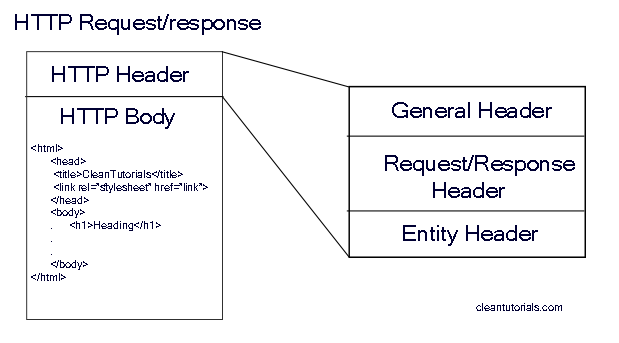
\includegraphics[width=0.618\textwidth]{graphics/http}
\end{figure}

\subsubsection{SSH}
\begin{figure}[H]
\centering
\resizebox{0.618\textwidth}{!}{\import{graphics/}{dns_format.pdf_tex}}
\end{figure}

\subsection{WIN-Kommandos}
\begin{description}
\item[ARP-Tabelle:]\begin{itemize}
                      \item arp -a (Tabelle anzeigen)
                      \item arp -d pc3 (Eintrag löschen)
                      \item arp -s pc3 0:0:c:e:12:37 (Eintrag hinzufügen)
                    \end{itemize}
\item[Routing Tabelle:] netstat -r
\item[Netzwerkinformationen:] ipconfig
\item[ping:] ping 8.8.8.8
\item[Weg eines Datenpaketes:] tracert
\end{description}

\subsection{Uni-, Multi-, Broadcast}\label{A4.9}
\begin{description}
        \item[Unicast:] Eine Nachricht wird an einen \emph{einzelnen Empfänger} gesendet
        \item[Multicast:] Eine Nachricht wird an eine ausgewählte \emph{Gruppe von Empfängern} gesendet (Vorteil: geringere Datenübertragungsrate notwendig, geringere Belastung des Mediums. Z.B. bei IP einstellbar über Adresse)
        \item[Broadcast:] Eine Nachricht wird an \emph{alle Teilnehmer} des Netzwerkes gesendet (sollte sich auf das eigende Netzsegment beschränken, d.h. nicht durch router weitergeroutet werden)
\end{description}

\pagebreak
\section{Versuchsaufgaben}
\subsection{Kennenlernen des Software-Analysators}
Nach Öffnen von Wireshark müssen die Capture-Optionen konfiguriert werden. Diese enthalten alle physischen und auch virtuellen Netzwerkschnittstellen. Es muss die Schnittstelle ausgewählt werden, deren Netzwerkverkehr der Analysator aufzeichnen soll. Zudem kann der \emph{Promiskuitive Modus} aktiviert werden, welcher dafür sorgt, dass auch Netzwerkverkehr aufgezeichnet wird, der nicht an die ausgewählte Schnittstelle gerichtet ist. Dies macht keinen Unterschied, wenn das Gerät an einen Switch angeschlossen ist, da dieser (i.d.R.) nur die wirkliche Zieladresse anspricht. In einem Funknetzwerk (WLAN) wäre der Mitschnitt des Verkehrs anderer mit dieser Einstellung jedoch möglich.\\

\begin{figure}[H]
  \begin{center}
      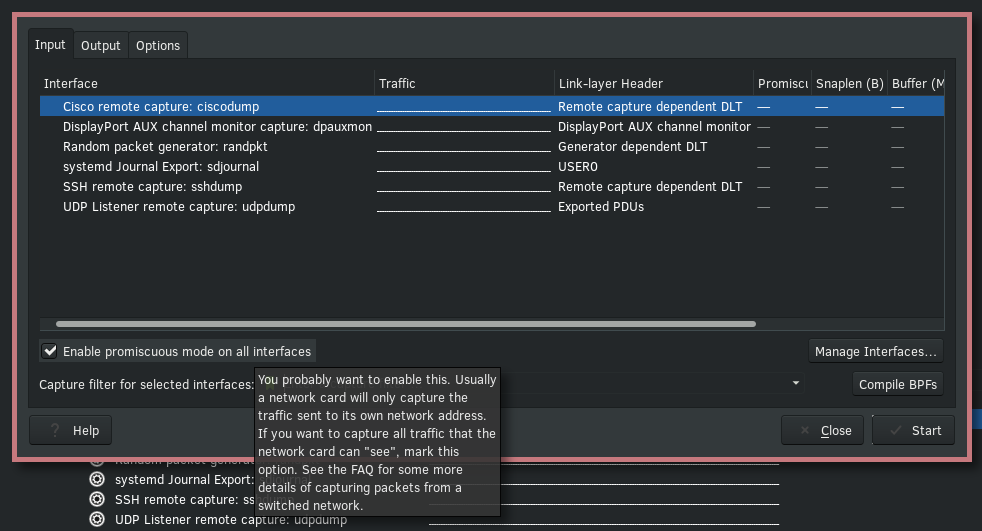
\includegraphics[width=0.618\textwidth]{graphics/capture_options.png}
      \caption{Auswahl der Netzwerkschnittstelle in den Capture-Optionen}
  \end{center}
\end{figure}

Im Optionen-Reiter der Capture-Optionen kann außerdem eingestellt werden, ob die angezeigten Adressen (MAC, Netwerk/IP, Transport) in Namen aufgelöst werden sollen (sofern möglich).\\

Nach der Aufzeichnung im Labor konnten die Daten als Trace-Dateien abgespeichert werden, um später analysiert zu werden. Zur Vereinfachung der Analyse kann man mithilfe von Filtern die Paketliste u.a. auf bestimmte Protokolle einschränken.
Beispielsweise wird mit dem Filter \inlinecode{tcp.port == 80} nur der Verkehr mit den TCP-Portnummern 80 (HTTP) angezeigt.


\subsection{Testen der Netzwerkkonfiguration}
\begin{figure}[H]
  \begin{center}
    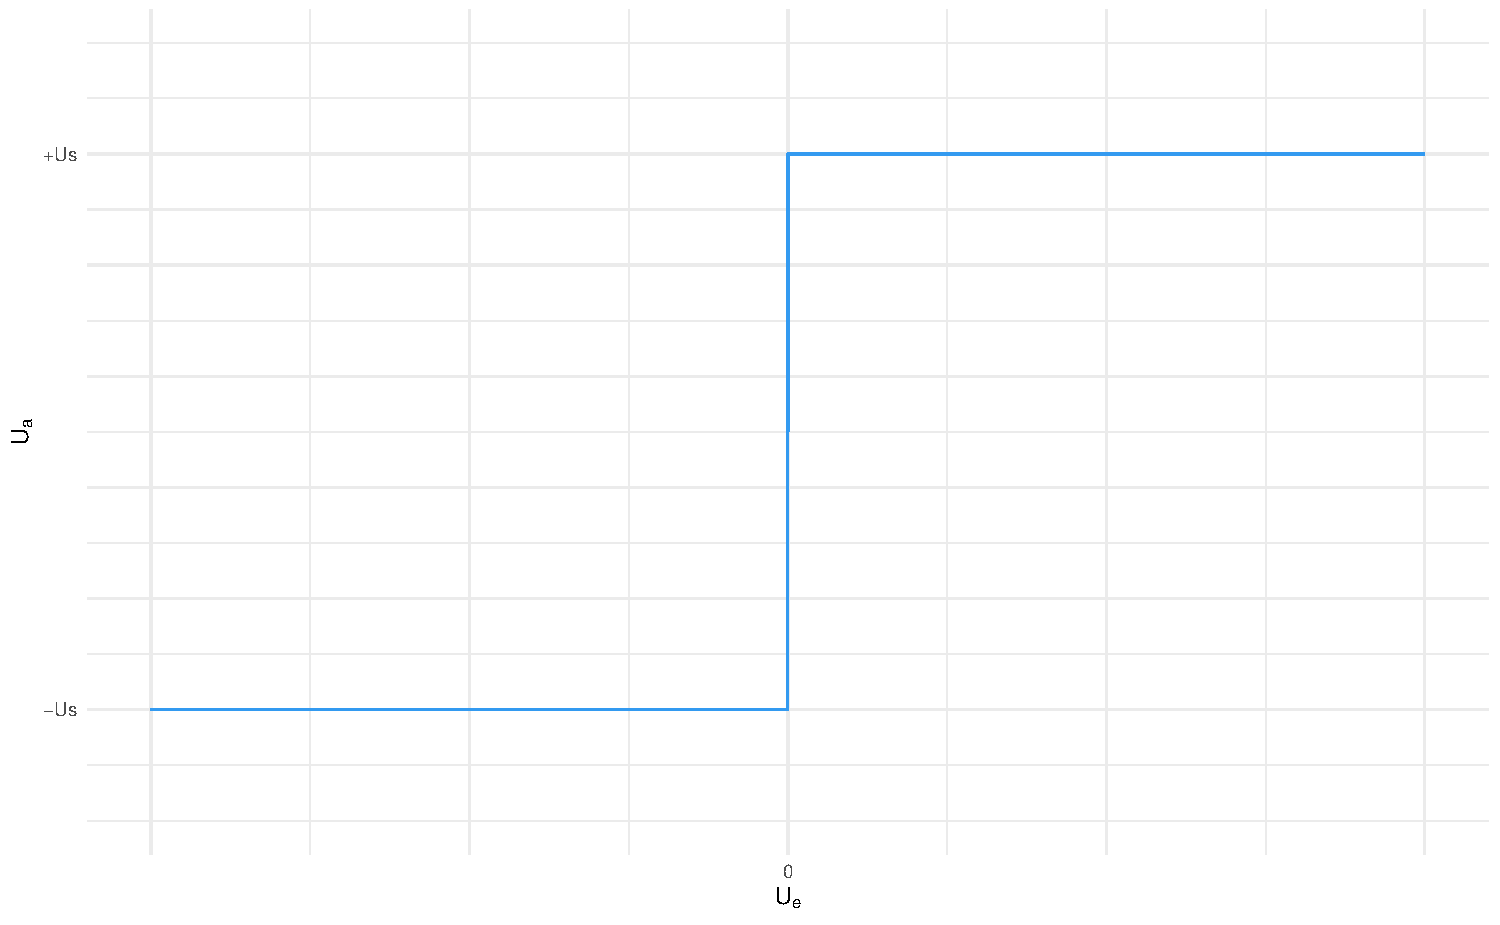
\includegraphics[width=0.618\textwidth]{1_2/opv_nofeed.pdf}
    \end{center}
    \caption{OPV-Kennlinie ohne Rückkopplung (ideal)}
 \end{figure}
\begin{figure}[H]
  \begin{center}
    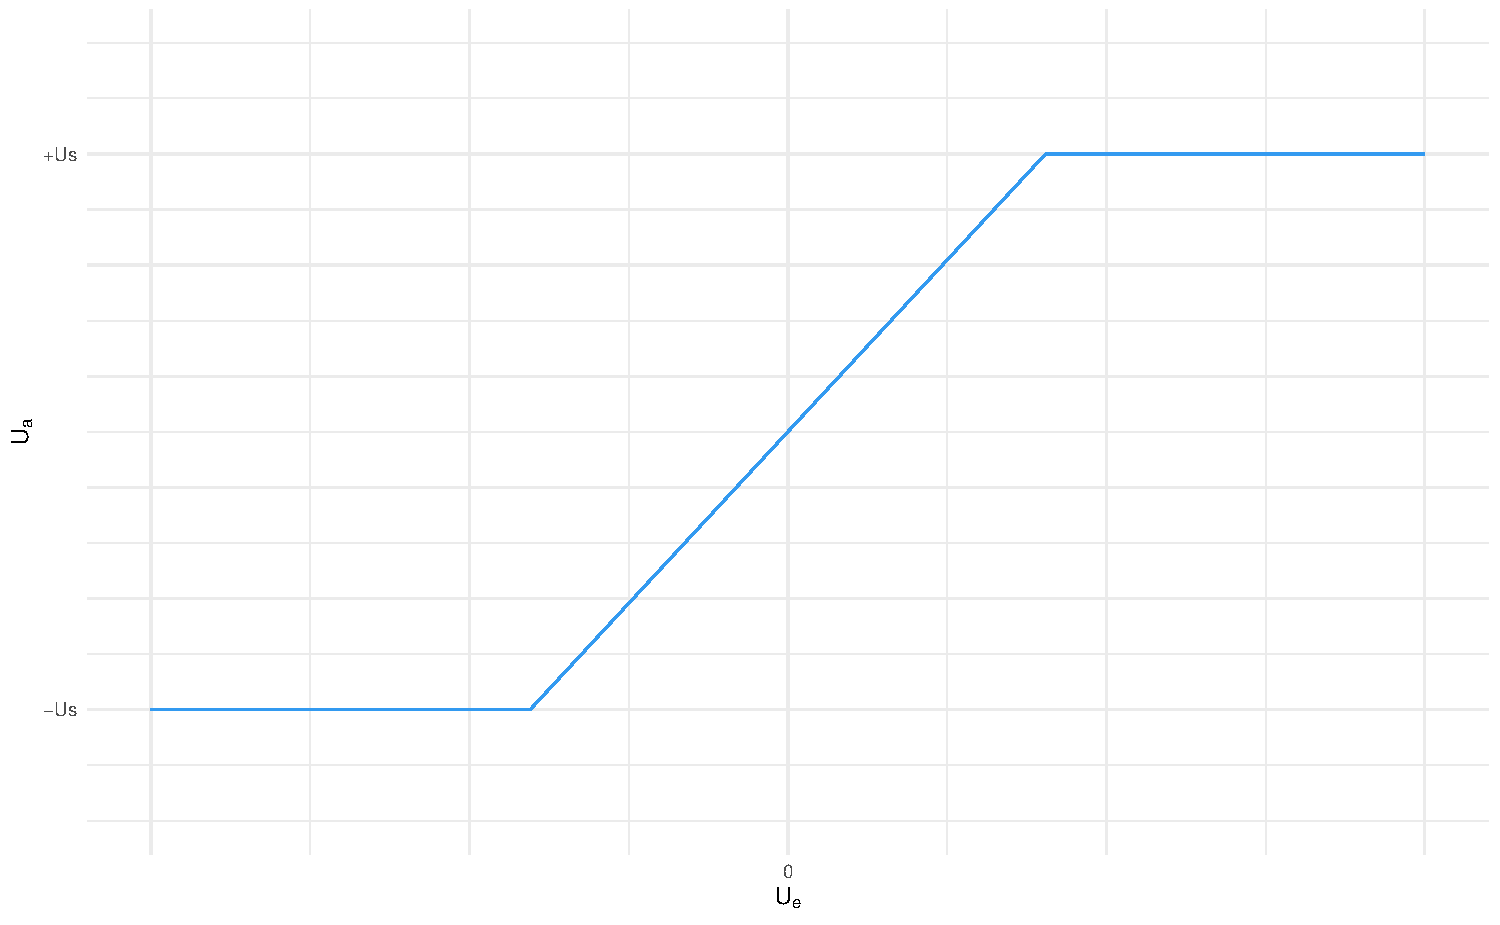
\includegraphics[width=0.618\textwidth]{1_2/opv_feed.pdf}
    \end{center}
    \caption{OPV-Kennlinie mit Rückkopplung}
 \end{figure}

Durch Rückführung eines Teils des Ausgangs- auf das Eingangssignal durch ein
Rückkopplungsnetzwerk wird der Operationsverstärker in einen linearen
Arbeitsbereich gebracht, wodurch die Verstärkung nicht mehr den Wert der der Leerlaufverstärkung (Abb. 1), sondern einen kontrollierten Verstärkungswert (Abb. 2) annimmt.


\subsection{Frameanalyse (Ethernet)}
Das Vierpolersatzschaltbild dient zur Kleinsignalbeschreibung des
Bipolartransistors. Die Kapaziäten im physikalischen Ersatzschaltbild führen zu
einer Frequenzabhängigkeit der Vierpolparameter.

\begin{figure}[H]
\begin{center}
\begin{circuitikz}

  \draw (-2,0) to[open, v=$u_1$] (-2,-4);
  \draw (9,0) to[open, v=$u_2$] (9,-4);

  \draw (-2,0) to [short, o-, i=$i_1$] (1,0)
              to [R, l=$h_{11}$] (1,-2)
              to [voltage source, l=$h_{12}\cdot u_2$, v_=$$, -*] (1,-4);

  \draw (5, -4) to[current source, l=$h_{21} \cdot i_1$, i=$$, *-] (5,0);
  \draw (6.618,0) to[R, l=$\dfrac{1}{h_{22}}$, *-*] (6.618, -4);


   \draw (-2,-4) to [short, o-o] (9,-4);
   \draw (5,0) to [short, -o] (9,0);
\end{circuitikz}
\caption{Hybridparametermodell}
\end{center}
\end{figure}
\[h_{11} \vcentcolon= \frac{u_1}{i_1}\rvert_{u_2=0}\]
\[h_{12} \vcentcolon= \frac{u_1}{u_2}\rvert_{i_1=0}\]
\[h_{21} \vcentcolon= \frac{i_2}{i_1}\rvert_{u_2=0}\]
\[h_{22} \vcentcolon= \frac{i_2}{u_2}\rvert_{i_1=0}\]


\begin{figure}[H]

\begin{center}
\begin{circuitikz}

  \draw (-3,0) to[open, v=$u_{BE}$] (-3,-4);
  \draw (9,0) to[open, v=$u_{CE}$] (9,-4);

  \draw (-3,0) to [short, o-, i=$i_1$] (1,0);
  \draw (0, 0) to [R, l_=$r_\pi$, *-*] (0,-4);
  \draw (1.382, 0) to [C, l=$C_{BE}$, *-*] (1.382,-4);

  \draw (1,0) to[C, l=$C_{BC}$] (5,0);

  \draw (5, -4) to[current source, l=$g_m u_{BE}$, i=$$, *-*] (5,0);
  \draw (6.618,0) to[R, l=$r_0$, *-*] (6.618, -4);


   \draw (-3,-4) to [short, o-o] (9,-4);
   \draw (5,0) to [short, -o] (9,0);
\end{circuitikz}
\end{center}
\caption{Kleinsignalersatzschaltbild des Bipolartransistors}
\end{figure}

\noindent Steilheit/Übertragungsleitwert:
\[ g_m = \frac{\dif I_{C}}{\dif U_{BE}} = \frac{I_{C,A}}{U_T} \]
Eingangswiderstand:
\[ r_\pi = \frac{\dif U_{BE}}{\dif I_B} = \frac{\beta_N}{g_m}= \frac{\beta_N \cdot U_T}{I_{C,A}} \]
Ausgangswiderstand ($U_{AN}:$ Early-Spannung):
\[r_0 = \frac{\dif U_{CE}}{\dif I_C} = \frac{U_{AN} + U_{CE,A}}{I_{C,A}}\]

\noindent Rückwärtssteilheit:
\[ \frac{\dif I_B}{\dif U_{CE}} \approx 0\]

\noindent $C_{BC}$: Sperrschichtkapazität (dominiert im normalen Verstärkerbetrieb)
\noindent $C_{BE}$: Diffusionskapaziät \\

\noindent Hybridparameter:

\begin{gather*}
  h_{11} \vcentcolon= \frac{u_1}{i_1}\rvert_{u_2=0}\\
  h_{11} = \frac{r_\pi \cdot \frac{1}{j\omega(C_{BE} + C_{BC})}}{r_\pi + \cdot
    \frac{1}{j\omega(C_{BE} + C_{BC})}} = \frac{r_\pi}{j\omega r_\pi
    (C_{BE}+C_{BC}) + 1}
\end{gather*}

\eqbox{
  h_{11} = r_\pi \cdot \frac{1}{1 + j\omega r_\pi(C_{BE} + C_{BC})}
}{0.618\textwidth}

\begin{gather*}
  h_{12} \vcentcolon= \frac{u_1}{u_2}\rvert_{i_1=0}\\
  i_1=0 \rightarrow i_B = 0 \rightarrow \beta_N \cdot i_B = 0 \rightarrow u_2 =
  0\\
\end{gather*}

\eqbox{
  h_{12} = 0
}{0.618\textwidth}

\begin{gather*}
  h_{21} \vcentcolon= \frac{i_2}{i_1}\rvert_{u_2=0}\\
  i_1 = \frac{u_{BE}}{r_\pi//(\frac{1}{j\omega(C_{BC}+C_{BE})})}\\
  i_2 = i_c = g_m \cdot u_{BE} = \frac{\beta_N}{r_\pi}\cdot u_{BE}\\
  \frac{1}{h_{21}} = \dfrac{\frac{u_{BE}}{\dfrac{r_\pi \cdot
      \frac{1}{j\omega(C_{BC}+C_{BE})}}{r_\pi +
      \frac{1}{j\omega(C_{BC}+C_{BE}}}} } { \dfrac{\beta_N}{r_\pi} \cdot u_{BE}}
 = \dfrac{\frac{1}{\dfrac{
      \frac{1}{j\omega(C_{BC}+C_{BE})}}{r_\pi +
      \frac{1}{j\omega(C_{BC}+C_{BE}}}} } { \beta_N }
 = \dfrac{\dfrac{
     1}{\frac{1}{r_\pi \cdot j\omega(C_{BC}+C_{BE}) + 1}} } { \beta_N }\\
 = \frac{1}{\beta_N \cdot \dfrac{1}{r_\pi \cdot j\omega(C_{BC}+C_{BE})+1}}\\
\end{gather*}
\vspace{-1cm}
\eqbox{
h_{21}=\beta_N \cdot \frac{1}{1 + j\omega r_\pi (C_{BC}+C_{BE})}}{0.618\textwidth}
($\omega \rightarrow 0 \rightarrow h_{21} = \beta_N$ )

\begin{gather*}
  h_{22} \vcentcolon= \frac{i_2}{u_2}\rvert_{i_1=0}\\
  \frac{1}{h_{22}}=r_0//\left(\frac{1}{j\omega C_{BC}} + (r_\pi //
    \frac{1}{j\omega C_{BE}})\right)\\
  = r_0 // \left( \frac{1}{j\omega C_{BC}} + \dfrac{1}{\frac{1}{r_\pi} + j\omega C_{BE}} \right)\\
  = \frac{r_0 \cdot \left( \dfrac{1}{j\omega C_{BC}} + \dfrac{1}{\frac{1}{r_\pi}
        + j\omega C_{BE}} \right)}{ r_0 + \left( \dfrac{1}{j\omega C_{BC}} +
      \dfrac{1}{\frac{1}{r_\pi} + j\omega C_{BE}} \right)}
\end{gather*}

\eqbox{
  \frac{1}{h_{22}} = \dfrac{r_0}{1 + \dfrac{r_0}{\left( \dfrac{1}{j\omega C_{BC}}
        + \dfrac{1}{r_\pi + j\omega C_{BE}} \right)}}
}{0.618\textwidth}

\noindent y-Parameter:
\begin{gather*}
  y_{11}=\frac{1}{h_{11}}\\
  y_{12}=\frac{-h_{12}}{h_{11}}\\
  y_{21}=\frac{h_{21}}{h_{11}}\\
  y_{22}=\frac{\textrm{det} H }{h_{11}}
\end{gather*}

\subsection{Analyse der Internetsitzungen}
\begin{figure}[H]
  \begin{center}
    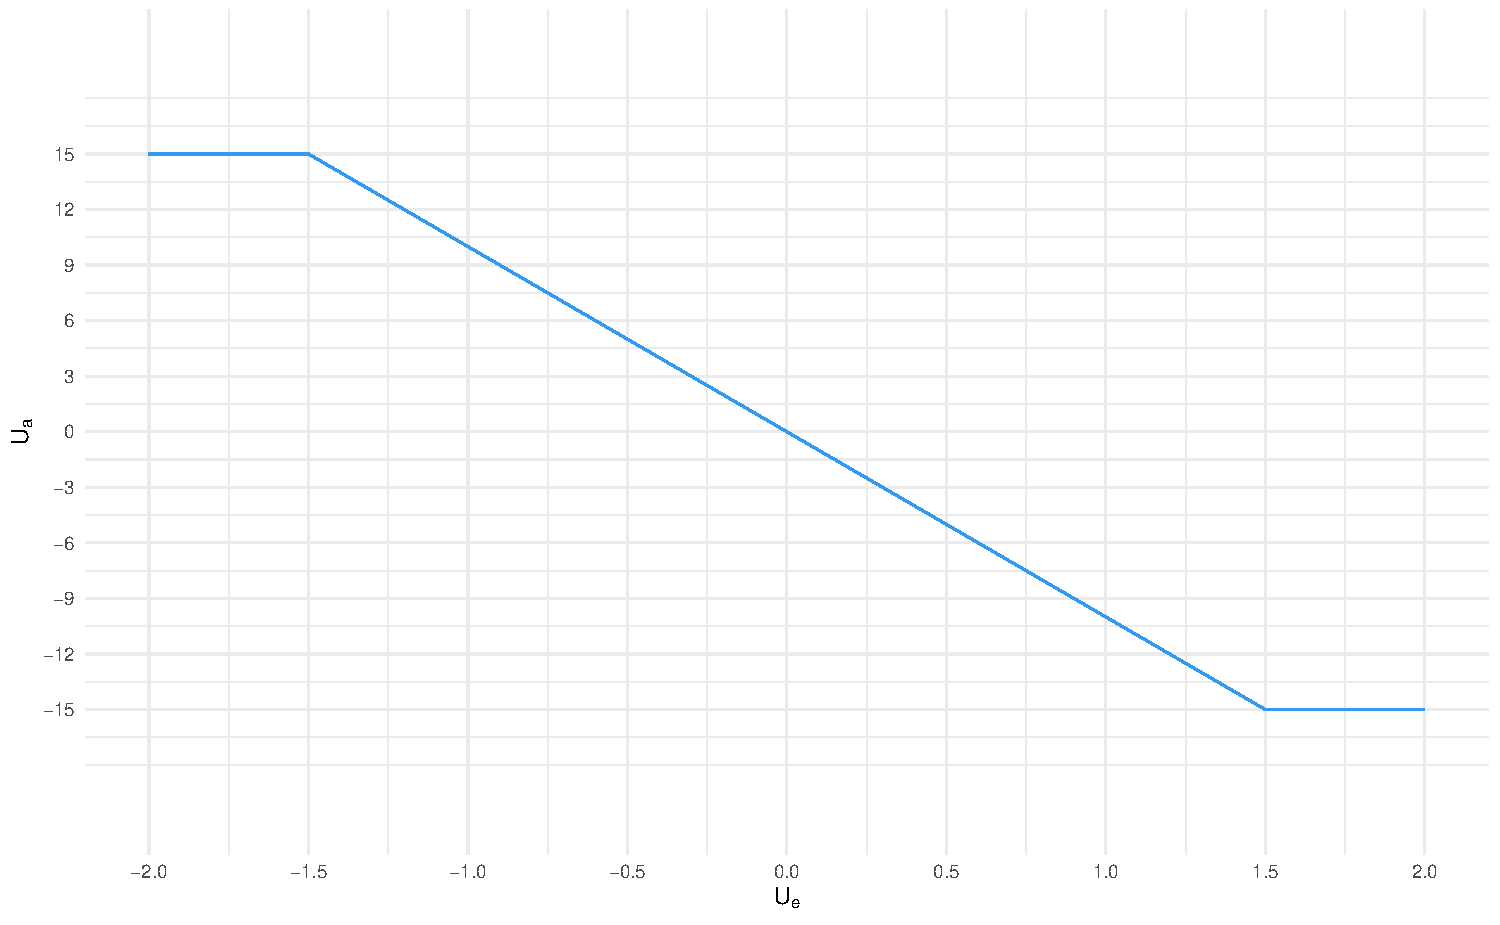
\includegraphics[width=\textwidth]{1_4/opv_inv_verst.pdf}
    \end{center}
    \caption{Kennlinie einer invertierenden OPV-Verstärkerschaltung mit einer Verstärkung von $V_u = -10$ und einer
      Versorgungsspannung von $U_s = \pm 15 \, \si{\volt}$}
 \end{figure}

Im ersten Schritt wurden ARP- und DNS-Cache geleert, um entsprechende Anfragen in Wireshark sehen zu können.\\

Es wurden dann folgende Web-Seiten im \emph{Mozilla Firefox} Browser nacheinander aufgerufen:
\begin{center}
  \underline{acad-30.na.hs-wismar.de}\\
  sowie\\
  \underline{hermes.fiw.hs-wismar.de/comlab}
\end{center}

Währenddessen wurde mithilfe von Wireshark die Netzwerkkommunikation mitgeschnitten. Abb. \ref{wire_34} zeigt einen Ausschnitt aus der Tracedatei, für die Übersicht wurde der Filter \inlinecode{tcp || http || dns}  angewandt.

\begin{figure}[H]
  \centering
  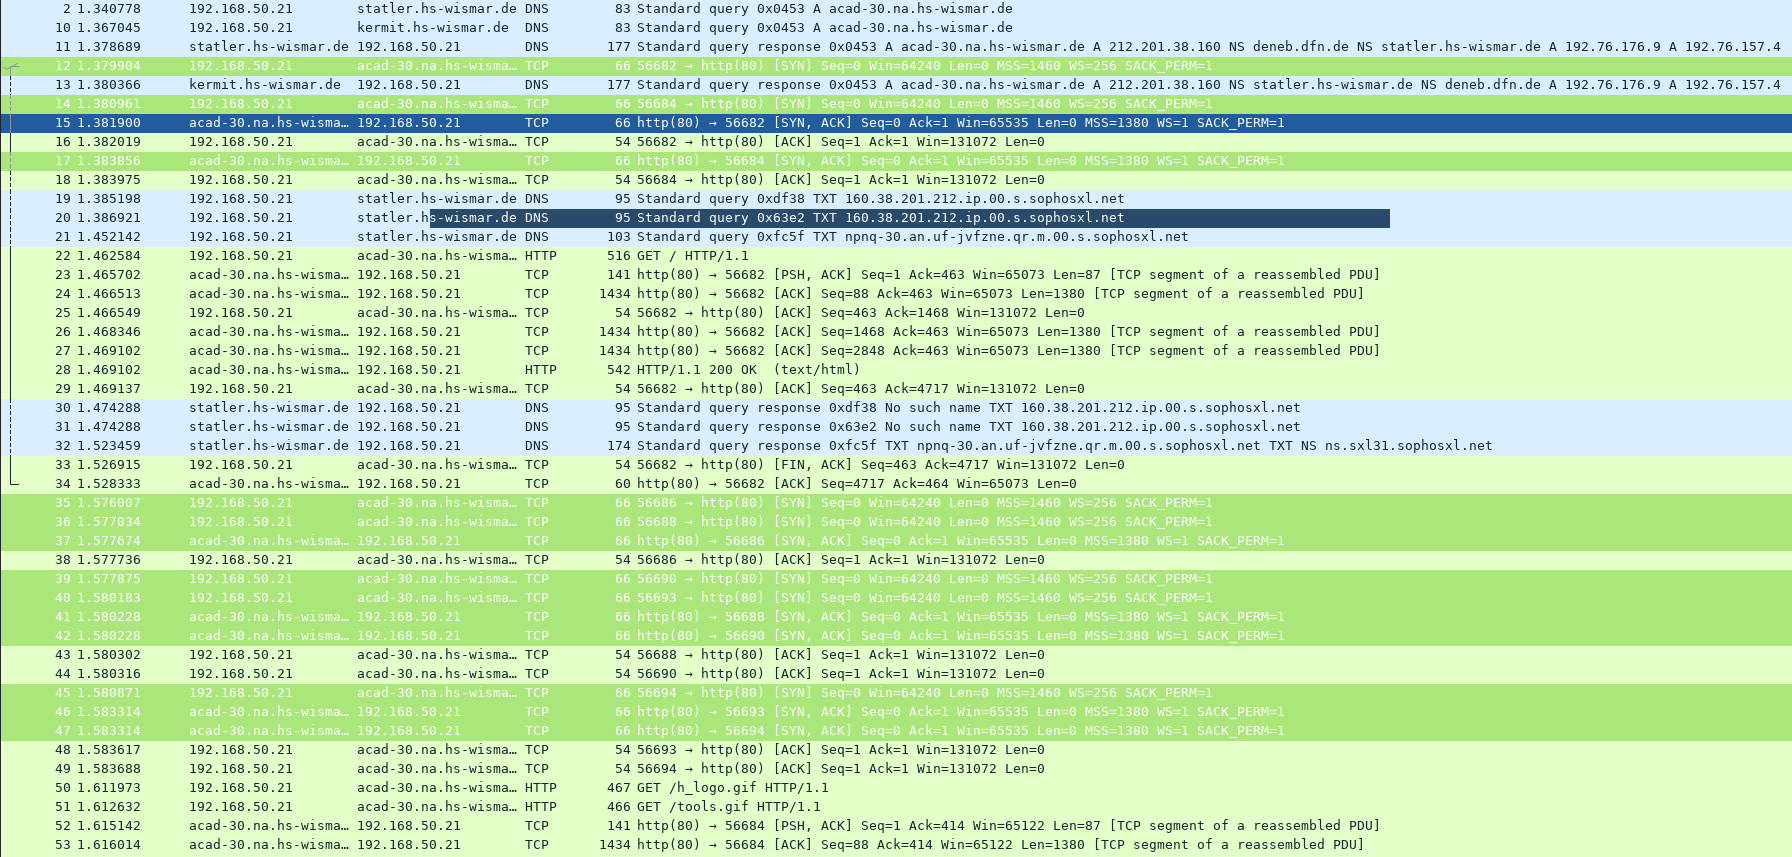
\includegraphics[width=\textwidth]{graphics/versuch/3_4/wireshark/trace_screenshot}
  \caption{Screenshot des Beginns des Wireshark-Mitschnittes, acad-30.na.hs-wismar.de (gefiltert)}\label{wire_34}
\end{figure}

\begin{figure}[H]
  \centering
  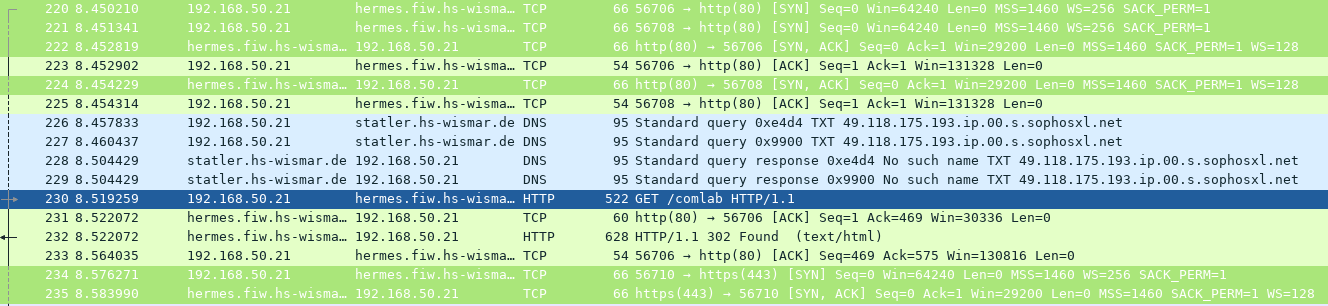
\includegraphics[width=\textwidth]{graphics/versuch/3_4/wireshark/wire_34_hermes}
  \caption{Screenshot des Beginns der Kommunikation mit hermes.fiw.hs-wismar.de (gefiltert)}\label{wire_34_hermes}
\end{figure}

\subsubsection{DNS-Anfragen}
Das DNS-Protokoll (Domain Name Service) ist ein Protokoll auf Anwendungsebene, das dafür zuständig ist, den jeweiligen Doimainnamen (z.B. acad-30.na.hs-wismar.de) in dessen IP-Adresse umzuwandeln. Ist diese Zuweisung nicht bereits im Zwischenspeicher vorhanden, muss der Client eine DNS-Anfrage an einen DNS-Server stellen. Dies passiert auch am Beginn der Kommunikatio, da der DNS-Cache im Vornherein gelöscht wurde (Abb. \ref{wire_34}).\\

Der Host \inlinecode{192.168.50.21}, auf dem der Name der Website in die Browserleiste eingegeben wurde, stellt eine Anfrage an den Server \emph{statler.hs-wismar.de} (\inlinecode{192.76.157.4}). Dieser befindet sich nicht im gleichen Subnetz, weshalb die Kommunikation über den Standardgateway (\inlinecode{192.168.50.1}) laufen muss, was auch durch das überprüfen der Ziel-MAC-Adresse im Ethernetframe zu erkennen ist.\\

Es sind keine weiteren ARP-Anfragen von der sendenden Schnittstelle notwendig, da die Hardwareadresse des Standardgateways anscheinend bekannt ist und weitere Hardwareadressauflösungen von den folgenden Netzwerkknoten gehandhabt werden.\\

Die DNS-Anfrage läuft über Ebene 4 mit dem verbindungslosen UDP-Protokoll zu Port 53 und enthält u.a. den ASCII-codierten Namen der Website, sowie bestimmte Flags, wie z.B. das Opcode-Flag 0 zur Signalisierung einer Anfrage (Abb. \ref{dns_request_acad}). Da es verbindungslos ist, sieht man beispielsweise auch keine Bestätigungsantworten (ACK), wie man es bei TCP erwarten würde.\\

Als Separator zwischen den URN-Bestandteilen ist in den eigentlichen Daten nicht der Punkt (wie man es im Browser eingibt), sondern der Hex-Wert \emph{02}, welcher im ASCII-Code für STX (Start of Text) steht (Abb. \ref{dns_request_acad} unten).

\begin{figure}[H]
  \centering
  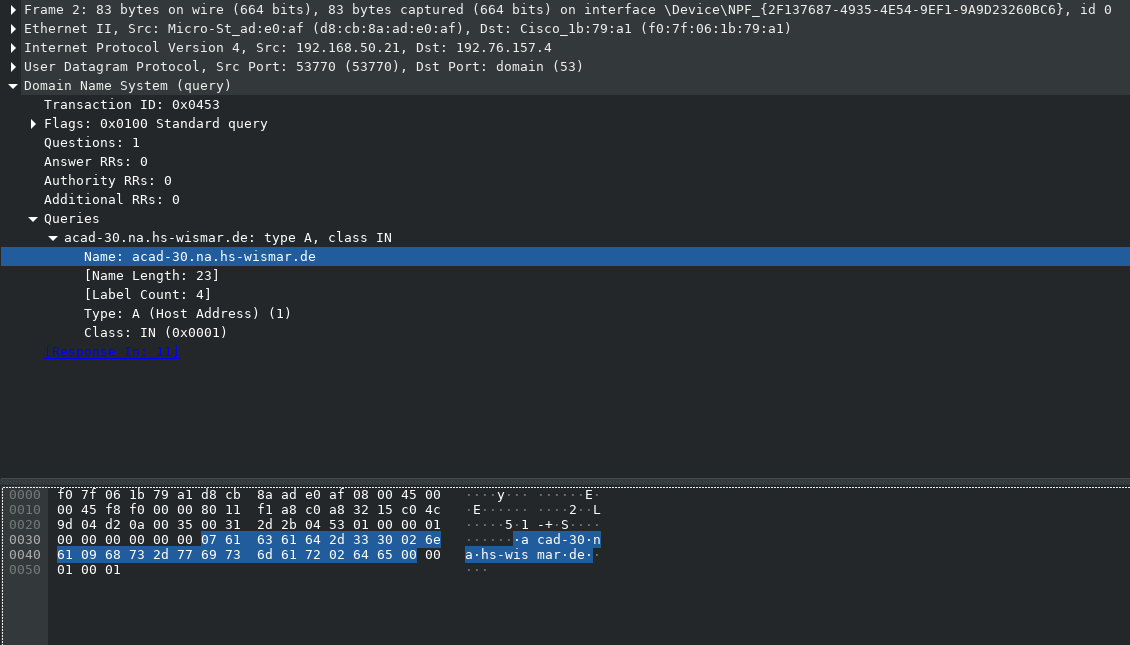
\includegraphics[width=\textwidth]{graphics/versuch/3_4/wireshark/dns_request}
  \caption{Erste DNS-Anfrage über acad-30.na.hs-wismar.de}\label{dns_request_acad}
\end{figure}

Es folgt in der nächsten Zeile eine weitere, parallele DNS-Anfrage an einen anderen Server (kermit.hs-wismar.de / \inlinecode{192.76.157.9}) zur Auflösung desselben Namens (acad-30.na.hs-wismar.de). Das geschieht möglicherweise, um im Fehlerfall des \glqq statler\grqq\ Servers trotzdem eine DNS-Auflösung zu erhalten.\\

Die Antwort auf die erste Anfrage erscheint nach etwa $38 \, \si{\milli\second}$. Sie enthält, wie erwartet, die zum Namen gehörende IP-Adresse \inlinecode{212.201.38.160}. Die Flags geben hier an, dass es sich um eine Standard-Antwort handelt und dass es keine Fehler gab (Abb. \ref{dns_reply_acad}).

\begin{figure}[H]
  \centering
  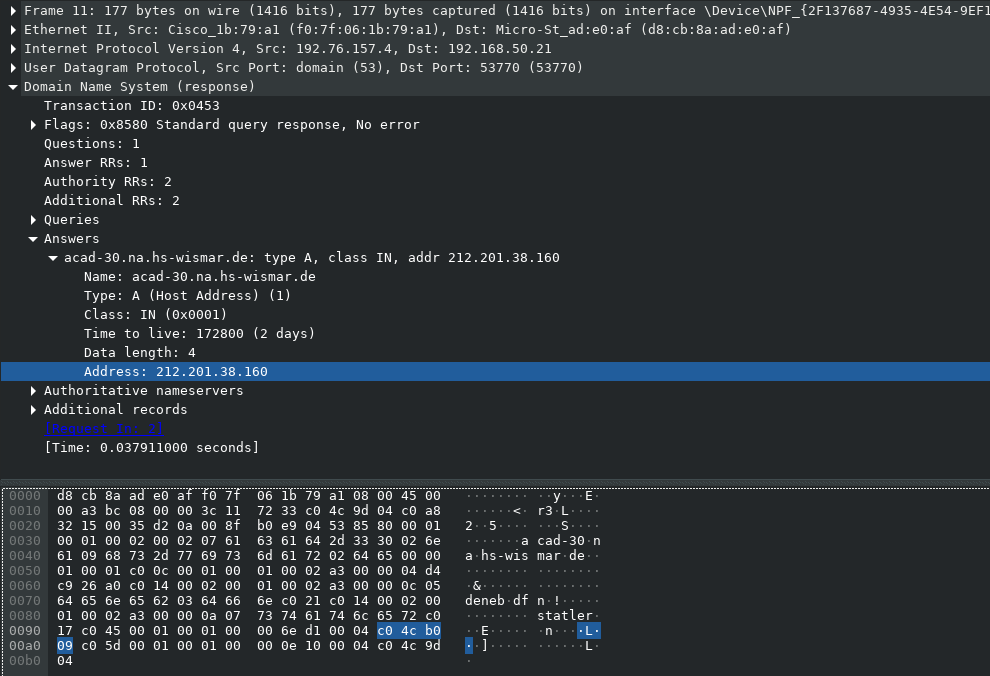
\includegraphics[width=\textwidth]{graphics/versuch/3_4/wireshark/dns_reply}
  \caption{Erste DNS-Antwort über acad-30.na.hs-wismar.de}\label{dns_reply_acad}
\end{figure}

\subsubsection{HTTP- und TCP-Verkehr}
Nach der Antwort wird die TCP-Kommunikation mit dem nun bekannten acad-30.hs-wismar.de auf Port 80 (HTTP) initiiert. Dies geschieht über den 3-Wege-Handshake (siehe \ref{three_way}). Der Sender legt einen zufälligen Port zur Identifizierung der Verbindung fest, welcher über dem sogenannten \glqq well known ports\grqq-Bereich (1024) liegt und kleiner als 65535 ist, in diesem Fall 56682.\\

Dann wird ein TCP-Paket mit gesetzem SYN-Bit (Synchronisation) an den Server geschickt, um diesem die eigene Sequenznummer (3291467299) für die Paketnummerierung, die Fenstergröße ($64240$) zur Flusskontrolle, sowie die maximale Segmentgröße (Datengröße) mitzuteilen. In Wireshark kann man für TCP-Streams relative Sequenznummern einstellen, wodurch die Nummerierung automatisch bei 0 beginnt (so auch in Abb. \ref{tcp_syn}). Außerdem wird während des Handshakes der Skalierungsfaktor für die Fenstergröße festgelegt. Dessen TCP-Feld ist 8, was einen Faktor von $2^{8} = 256 bedeutet$.\\

Kurz danach öffnet der Client einen weiteren Port (56684) für die TCP-Kommunikation mit dem gleichen Server auf Port 80. Er fährt dabei genauso vor wie bei der vorherigen Initiierung. Die parallelen Verbindungen werden dann genutzt, um jeweils verschiedene Ressourcen vom Server \glqq gleichzeitig\grqq\ anzufragen (z.B. HTML, Bilder etc.).\\

Auf die erste SYN-Anfrage antwortet der Server in gleicher Weise mit einem TCP-Paket, in welchem das SYN-Bit sowie nun auch das ACK-Bit zur Bestätigung gesetzt sind. Der Server teilt dem Client ebenfalls seine Windowgröße ($65535 \cdot 1$), Sequenznummer (167188764) und maximale Segmentgröße (1380) mit und richtet sie an Port 56682.\\

Dazwischen erscheint noch die Antwort auf die zweite DNS-Anfrage von kermit.hs-wismar.de, welche wahrscheinlich ignoriert wird, da die Auflösung bereits bekannt ist.\\

Im dritten Schritt des three-way-handshakes erhält der Server vom Client ein ACK, um den Empfang des vorherigen TCP-Paketes zu bestätigen (Abb. \ref{tcp_ack}). Hierin ist die Sequenznummer auf 1 gesetzt, um zu kennzeichnen, dass das nächste Paket, das empfangen werden kann die (relative) Sequenznummer 1 besitzt. Man erkennt außerdem, dass die Fenstergröße nur 512 Byte beträgt. Da im Handshake allerdings der Fensterskalierungsfaktor 256 festgelegt wurde, ist die tatsächliche Fenstergröße $131072$, was auch im durch Wireshark hinzugefügten Feld [Calculated window size] zu sehen ist.\\

Der andere TCP-Handshake auf Client-Port 56684 verläuft analog.\\

\begin{figure}[H]
  \centering
  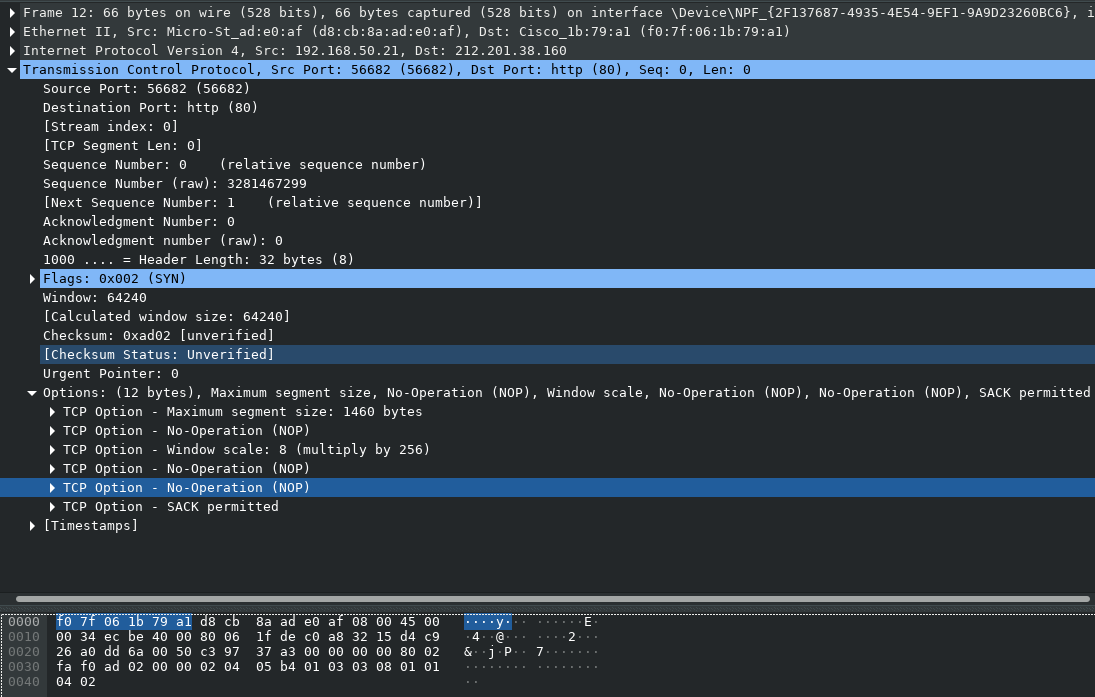
\includegraphics[width=\textwidth]{graphics/versuch/3_4/wireshark/tcp_syn}
  \caption{Erstes TCP-Paket für Three-Way-Handshake mit SYN-Bit}\label{tcp_syn}
\end{figure}

\begin{figure}[H]
  \centering
  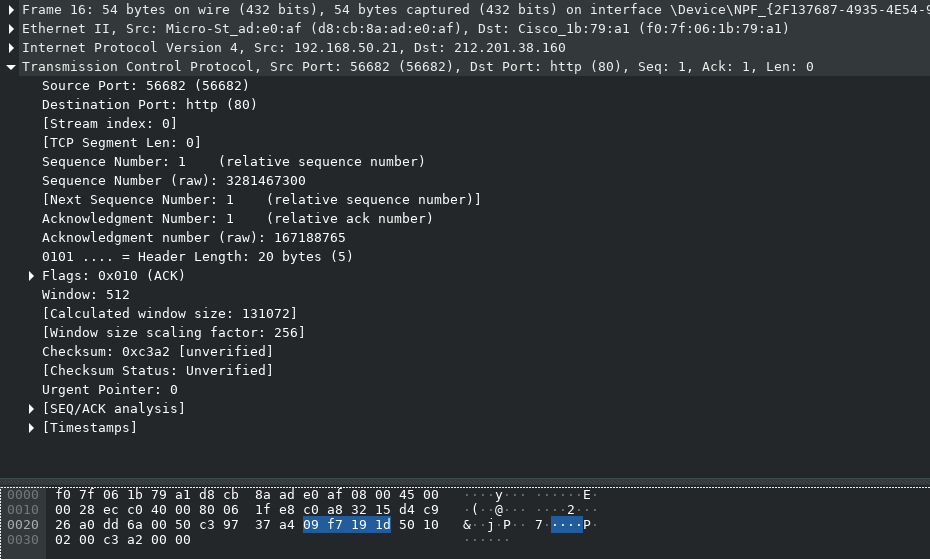
\includegraphics[width=\textwidth]{graphics/versuch/3_4/wireshark/tcp_ack}
  \caption{Beenden des Three-Way-Handshakes mit ACK}\label{tcp_ack}
\end{figure}

Vor der ersten HTTP-Anfrage erscheinen noch drei DNS-Anfragen zur Auflösung der Namen \glqq 160.38.201.212.ip.00.s.sophosxl.net\grqq\ sowie \glqq npnq-30.an.uf-jvfzne.qr.m.00.s.sophosxl.net\grqq\ an den Server \inlinecode{192.76.157.4}, welche jedoch, wie in der DNS-Antwort bei Nummern 30-32 zu sehen, von diesem nicht aufgelöst werden können.\\

\begin{figure}[H]
  \centering
  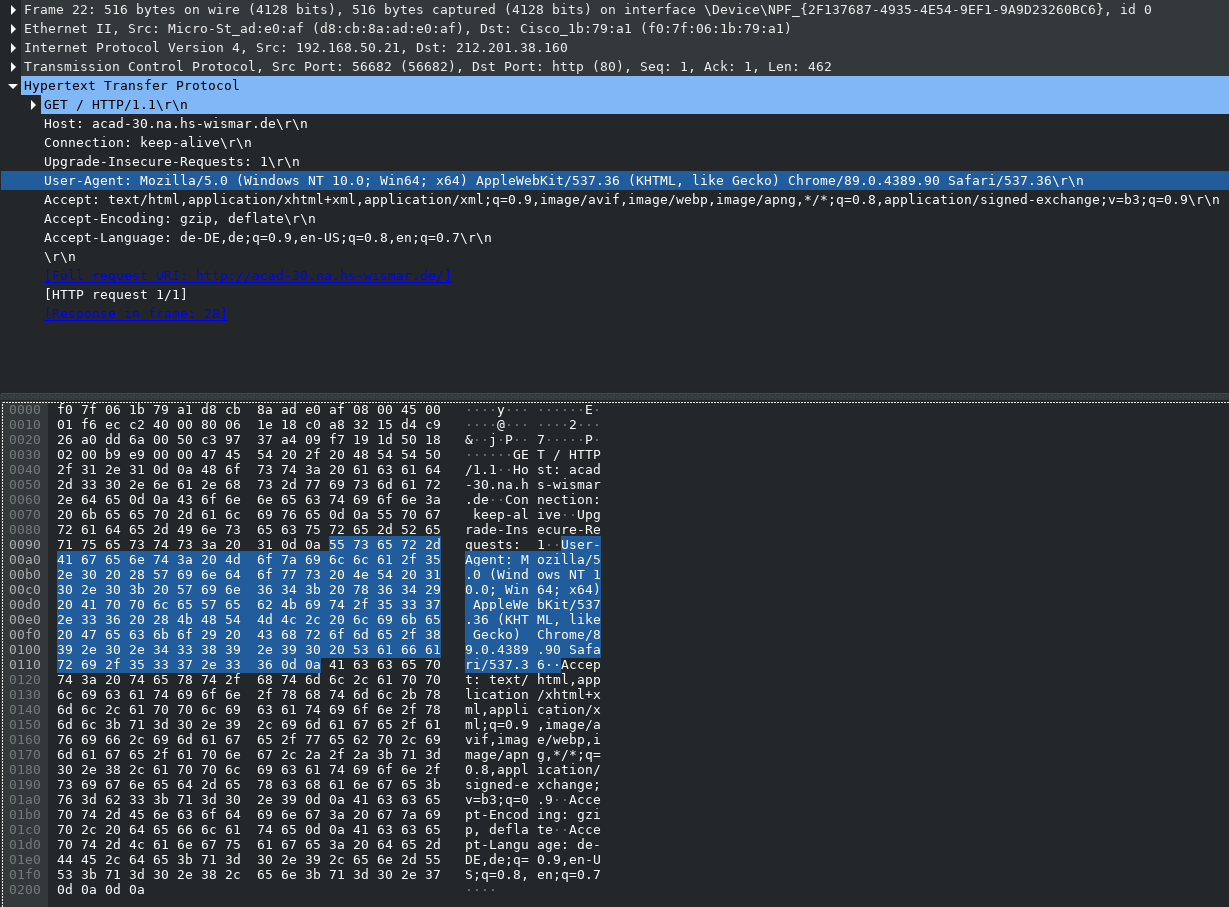
\includegraphics[width=\textwidth]{graphics/versuch/3_4/wireshark/http_request}
  \caption{HTML-Anfrage}\label{http_request}
\end{figure}

Es folgt die HTTP-Anfrage zum Grundverzeichnis der Website \glqq /\grqq\ . Diese enthält u.a. Informationen über Sprache, Kodierung, Browser und Plattform. Sie wird vom Server sofort zusammen mit den ersten Daten bestätigt. Da die maximale Segmentgröße (MSS) beim Handshake zu 1380 Byte festgelegt wurde, können die Daten nicht als ein einziges Segment verschickt werden, sondern müssen in maximal dieser Größe segmentiert sein. In Abb. \ref{wire_34} ab Paket 23 erkennt man dieses Verhalten. Zuerst werden Daten der Länge 84, dann Daten der Länge 1380 übertragen, also insgesamt 1467 Byte. Dies überschreitet zwar noch nicht die festgelegte Fenstergröße, allerdings ist das nur die maximale Grenze und nach Konvention wird jedes zweite (oder spätere) Paket bereits mit einem ACK bestätigt, wie bei Paket 25 zu sehen. Wireshark kennzeichnet TCP Segmente, die zu größeren, zusammenhängenden Daten gehören außerdem als [TCP segment of a reassembled PDU].\\

Der HTML-Status \glqq 200 OK\grqq\ wird dann gesendet, um eine erfolgreiche Anfrage zu signalisieren. Der Client bestätigt folglich noch das Empfangen der Daten.\\

Auf diese Weise wurde eine 4715 Byte große HTML-Datei übertragen, welche der Browser dann darstellen kann. Diese kann man auch erkennen, wenn man sich die (zusammengesetzten) Daten der Pakete anschaut.\\

Von der Server-Seite wird mit dem letzen HTTP-Paket mittels [FIN, ACK] das Kommunikationsende auf dem Port 80/56682 angefragt, was dann vom Client mit einem [FIN, ACK] bestätigt wird, worauf der Server erneut mit einem ACK antwortet.\\

Später wird noch eine Datei \emph{h\_logo.gif}, also eine Bilddatei im GIF-Format, angefragt und auch übertragen (Abb. \ref{gif_data}). Man kann die gesendeten Daten mit Wireshark extrahieren und wieder zusammensetzen. Dazu geht man auf File $\rightarrow$ Export Objects $\rightarrow$ HTTP und wählt die entsprechende Datei aus. Das Ergebnis ist in Abb. \ref{hlogo} zu sehen.

\begin{figure}[H]
  \centering
  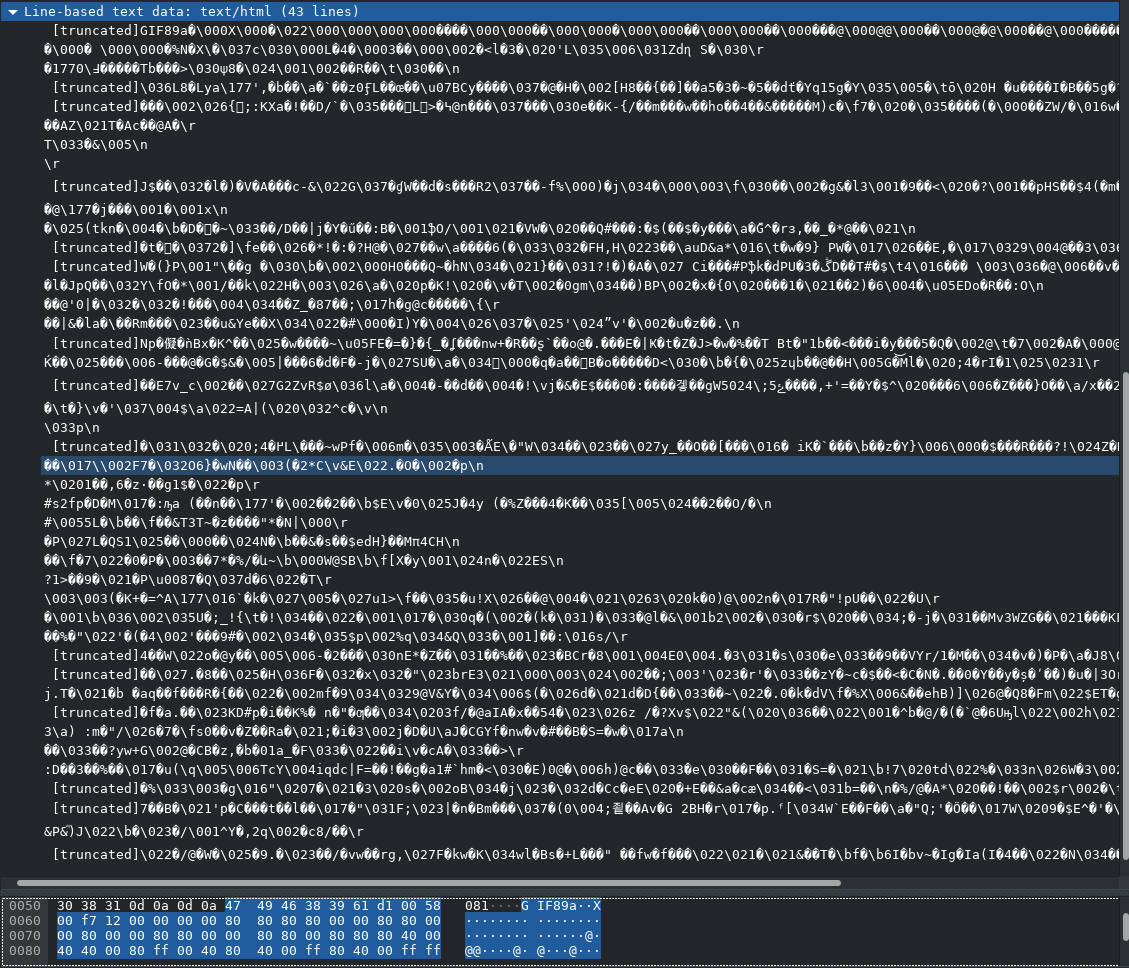
\includegraphics[width=\textwidth]{graphics/versuch/3_4/wireshark/gif_data}
  \caption{Ausschnitt aus dem HTTP-Paket für die Datei h\_logo.gif}\label{gif_data}
\end{figure}

\begin{figure}[H]
  \centering
  
\includegraphics[width=\textwidth]{graphics/versuch/3_4/wireshark/h_logo}
  \caption{Entnommene GIF-Datei}\label{hlogo}
\end{figure}

\subsubsection{Flussdiagramm der Sitzungen}
Da die Kommunikation aus vielen HTTP-Anfragen besteht, wurden in den Flussdiagrammen jeweils nur die DNS-Anfragen und die ersten TCP-Verbindungen bis zu deren Ende (FIN) dargestellt. Außerdem wurden nur die \glqq höchsten\grqq\ Protokolle in den jeweiligen Paketen gekennzeichnet (z.B. HTTP, obwohl es natürlich in einem TCP Paket eingebettet ist).

\begin{figure}[H]
\centering
\resizebox{0.618\textwidth}{!}{\import{graphics/}{acad_flowchart.pdf_tex}}
\caption{Flussdiagramm der Verbindung mit acad-30.na.hs-wismar.de}
\end{figure}

\begin{figure}[H]
\centering
\resizebox{0.618\textwidth}{!}{\import{graphics/}{hermes_flowchart.pdf_tex}}
\caption{Flussdiagramm der Verbindung mit hermes.fiw.hs-wismar.de}
\end{figure}

\end{document}
